\documentclass[11pt,conference,compsocconf]{IEEEtran}

\usepackage{hyperref}
\usepackage{graphicx}	% For figure environment
\usepackage[english]{babel}
\usepackage{tabu}
\usepackage{xargs}  
\usepackage{float}
\usepackage[prependcaption,textsize=tiny]{todonotes}
\presetkeys{todonotes}{inline,backgroundcolor=red}{}


\begin{document}
\title{Class Project 2 Report: Road Segmentation Challenge}

\author{
  Angerand Gr\'egoire, Goullet Boris, Grondier Julien 
}

\maketitle

\begin{abstract}
In this project, we were given a dataset consisting of aerial photographs of suburban areas. Our task was to apply different machine learning methods to this dataset to train a model that would predict where roads were present in these photographs.

\todo{summarize results}
\end{abstract}


\section{Models applied}

\subsection{Logistic regression}
At first, we tried using a logistic regression. We did this by cutting up the images into small patches (either 4x4, 8x8, or 16x16) and training a logist model on 3 features for that patch: mean Red pixels values, mean Green pixel values, and mean Blue pixel values.

However, results were less than satisfactory, even with more/different features or patch sizes, so we quickly dropped that idea.

\subsection{Convolutional Neural Network}
Started off by using the given tensorflow network

\subsubsection{Custom CNN classifier}
We tried building our own Convolution Neural Network rather than using the provided one, for better modularity. We were aiming for the following architecture: 

\begin{figure}[h]
\centering
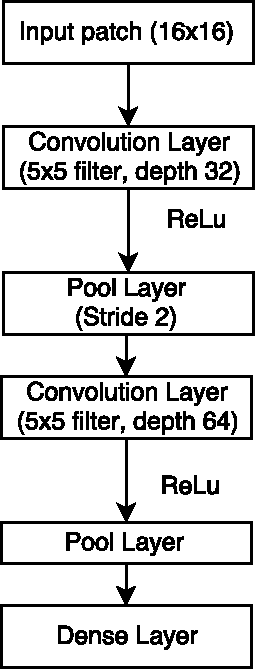
\includegraphics[width=\linewidth,height=0.5\textheight,keepaspectratio]{custom_CNN.pdf}
\caption{Architecture of our attempted custom CNN}
\end{figure}

However, after a lot of debugging, we failed to achieve anything and had to fallback on the provided file. The code can be checked in custom\_classifier.py

\section{Feature pre-processing}

Our CNN works on sub-patches of 4x4x3 (RGB) of the training images with labels from the corresponding ``groundtruth'' patch.

We train the CNN by cutting up 500 different source images: the 100 given as a dataset, plus variations of those (transposed, flipped horizontally, flipped vertically, and flipped both vertically and horizontally).

Furthermore, we tried adding a new label as groundtruth, manually annotated, corresponding the the position of roofs. However, this did not improve prediction rate compared to having only `background' and `road' as labels.


\section{Results post-processing}
After obtaining the raw prediction from the convolutional neural network, we do a post-processing step in order to remove most of the noise.

The post processing consists of a series of convolutions, using a cross shaped kernel. This shape has be chosen to match the many right angle intersections present in our dataset.

In some cases the roads are not aligned to the image axes, to handle those we extract the most significant straight lines from the image using Hough transform and rotate our kernel to match their orientation.


\section{Discussion}


\section{Summary}
While we had high hopes for using a custom CNN architecture, we are disappointed that we weren't able to build a functional one. However, using the basic, provided CNN, we achieved results that we would deem satisfactory

\end{document}
